% -----------------------------------------------------------------
% => INTRODUCTION - 1
% -----------------------------------------------------------------
\chapter{Introdução} \label{Chap:intro}

Na sociedade atual, os artefatos tecnológicos são parte integrante da vida das pessoas, moldando seu relacionamento consigo mesmas e com o mundo~\citep{Leitao:2014}. Além disso, a possibilidade de armazenar e analisar grandes volumes de dados tem permitido que tecnologias baseadas em Inteligência Artificial (IA) sejam cada vez mais utilizadas para melhorar processos nos mais diversos setores da sociedade, facilitando tomadas de decisões e reduzindo desperdícios de recursos. Assim, em 2011, na Feira de Hannover (Alemanha) cunhou-se o termo ``Indústria 4.0'' que denomina uma Quarta Revolução Industrial, cujo objetivo é tornar os processos industriais mais inteligentes e autônomos utilizando, dentre outras coisas, Inteligência Artificial, Sistemas Ciber-Físicos (CPS) e a emergente Internet das Coisas (IoT)~\citep{MCDIC:2014, Almeida:2018}.

%Segundo \cite{bassedas:1996}, o objetivo da escola, enquanto instituição, é a educação dos alunos que, para ele, significa a transmissão e o ensino de conteúdos determinados. Num sentido amplo, esses conteúdos seriam conceitos, acontecimentos, procedimentos, atitudes, valores e normas. Desse modo, pode-se afirmar que a função principal da escola é introduzir o indivíduo na sociedade.

Para cumprir mais eficazmente o seu papel de integração e socialização da cultura e do conhecimento, a escola não teria como passar imune a essa nova revolução~\citep{Nogueira:2013, Levy:2010}. Assim, a escola precisa, não somente inserir recursos tecnológicos dentro dos processos de ensino-aprendizagem, mas, propor novas metodologias e práticas pedagógicas~\citep{Sousa:2011} que, integradas às novas tecnologias, ajudem os alunos a desenvolver as competências e habilidades necessárias a dinamicidade do novo mundo a partir da nova revolução industrial~\citep{Fuhr:2018}, isto é, ultrapassando a noção de educação como mera aquisição de conhecimento fechado e em escala industrial, proveniente das duas primeiras revoluções industriais~\citep{Intelitek:2018}.

% A sociedade atual é profundamente marcada pela tecnologia, o que implica que os artefatos tecnológicos não são tratados como simples ferramentas, mas, como parte integrante da vida das pessoas, moldando o modo como elas se relacionam consigo mesmas e com o mundo ao seu redor \citep{EspiritoSanto:2012,Leitao:2014}. Assim, para cumprir mais eficazmente a sua função social, a escola precisa integrar os recursos tecnológicos nos processos de ensino propondo novas metodologias e práticas pedagógicas \citep{Sousa:2011}.

Essa demanda de integração da tecnologia nos ambientes educacionais tem possibilitado a construção de novos cenários de aprendizagem e a utilização de ferramentas que colaborem, tanto com os processos de ensino quanto de avaliação do desempenho dos estudantes, através do reconhecimento de contextos, atividades ou comportamentos dos estudantes durante a aula e, assim, façam recomendações com o objetivo de melhorar a qualidade da educação~\citep{Cheng:2006,Dong:2007,Mathioudakis:2013}. Tal integração pode envolver aplicações dos conceitos de Internet das Coisas, Inteligência Ambiental ({\it Ambient Intelligence}), Aprendizagem Ubíqua, Ciência de Contexto ({\it context-awareness}), Sistemas Multiagente e Sistemas Ciberfísicos~\citep{Oluwagbemi:2014,Xue:2011} e tem sido chamada de \textbf{Educação 4.0}~\citep{Hussin2018}.

Além disso, especialmente relacionado aos sistemas ciberfísicos, é importante destacar que a integração de interfaces tangíveis (Seção~\ref{section:TUI}) em ambientes de aprendizagem, tornando-os ambientes tangíveis, adicionam novas perspectivas ao processo de ensino-aprendizagem, uma vez que a metodologia pedagógica pode ser expandida para além dos objetos de aprendizagem tradicionais (baseados apenas em interação virtual), passando a incluir também manipulativos físicos dentro de um horizonte computacional.

% Entretanto, apenas criar ou utilizar recursos educacionais tecnológicos não garante a eficácia e nem a melhoria da qualidade da educação, pois, o aproveitamento de uma aula está relacionado ao engajamento do aluno no processo de ensino-aprendizagem. Assim, o uso de tecnologias em sala de aula também poderia permitir inferências como engajamento, nível de entendimento e dificuldades dos estudantes ao longo de um processo educativo~\citep{Gligoric:2015,Leitao:2015}. Tais inferências podem auxiliar o professor na criação ou modificação de conteúdos educacionais mais adequados ao perfil e necessidades de uma turma ou de um estudante.

% -----------------------------------------------------------------
% => CONTEXTO
% -----------------------------------------------------------------
\section{Contexto}
\label{section:contexto}

Segundo \cite{bassedas:1996}, o objetivo da escola, enquanto instituição, é a educação dos alunos que, para ele, significa a transmissão e o ensino de conteúdos determinados. Num sentido amplo, esses conteúdos seriam conceitos, acontecimentos, procedimentos, atitudes, valores e normas. Desse modo, pode-se afirmar que a função principal da escola é introduzir o indivíduo na sociedade.

Além disso, para o sociólogo da educação Pierre Bourdieu, o sucesso  escolar do estudante depende de levar em consideração a bagagem que ele traz consigo~\citep{Nogueira:2013}. Desse modo, o uso de um determinado capital cultural (por exemplo, o uso de dispositivos móveis e da internet) previamente pertencente ao estudante facilitaria o processo de ensino-aprendizagem dos códigos e conteúdos transmitidos pela escola formal. Além disso, para \cite{bassedas:1996}, tal processo possui três elementos: o estudante, os conteúdos de aprendizagem e o professor.

% Assim, para melhoria e maior eficiência do processo de ensino-aprendizagem, é preciso levar em consideração a grande familiaridade que as crianças e jovens tem com as novas tecnologias e inseri-las definitivamente na educação. Por isso, este trabalho está situado no contexto do desenvolvimento de ambientes de sala de aula inteligente com enfoque na utilização de objetos de aprendizagem físico-virtuais (com interfaces concretas e virtuais integradas) como ferramenta de apoio aos processos de ensino e de avaliação da aprendizagem.

%anterior Assim, tendo em vista as infinitas possibilidades que emergem da Educação 4.0, este trabalho está situado no contexto do desenvolvimento de ambientes físico-virtuais de aprendizagem com enfoque na utilização de ferramentas de apoio às atividades do professor e do estudante. No lado do professor, o suporte acontece na geração, uso e avaliação de materiais didáticos e desempenho dos estudantes. No lado do estudante, a novidade está na inserção de ferramentas e objetos de aprendizagem físico-virtuais que se adaptem às suas necessidades e ao ambiente, possibilitando que o mesmo possa construir experiências que levem à construção de conhecimento.

%atual
Assim, tendo em vista as infinitas possibilidades que emergem da Educação 4.0, este trabalho está situado no contexto do desenvolvimento de ambientes tangíveis de aprendizagem com enfoque na utilização de ferramentas de apoio às atividades do professor e do estudante. No lado do professor, a novidade está na geração e no uso de materiais didáticos diferenciados que possibilitem inclusive uma avaliação da aprendizagem dos estudantes. No lado do estudante, a novidade está na inserção de ferramentas e objetos tangíveis de aprendizagem que sejam mais interessantes do que o ensino tradicional, possibilitando que o mesmo possa executar atividades que levem à construção de conhecimento.

%anterior Como ponto de partida, tem sido aprimorada uma plataforma implementada ao longo do projeto de mestrado do proponente, a qual é composta de quatro partes: (i) Compositor, que é uma ferramenta para geração de material didático a partir de objetos de aprendizagem inseridos pelo professor ou provenientes de um repositório; (ii) Player, que propõe uma interface multiplataforma responsável pela execução da aula em dispositivo portátil, incluindo possibilidades de interação físico-virtual; (iii) Servidor, que é responsável pela criação, gerenciamento da sala de aula e adaptação do conteúdo educacional a partir das análises feitas dos dados obtidos da interação do estudante com o conteúdo educacional; e (iv) Analytics, que é responsável pela análise de dados para tomadas de decisão e geração de gráficos que auxiliem o professor na percepção do impacto de determinada atividade educacional na turma e futuras tomadas de decisões metodológicas. Tais ferramentas serão melhor apresentadas ao longo desta proposta, onde também serão introduzidas as futuras modificações para implementação do novo sistema.

Como ponto de partida, foi aprimorada uma plataforma inicialmente proposta na dissertação de mestrado de \cite{leitao:2017}, a qual é composta de quatro partes: (i) Compositor, que é uma ferramenta para geração de material didático a partir de objetos de aprendizagem inseridos pelo professor ou provenientes de um repositório; (ii) Player, que propõe uma interface multiplataforma responsável pela execução da aula em dispositivo portátil, incluindo possibilidades de interação tangível; (iii) Servidor, que é responsável pela criação, gerenciamento da sala de aula, exibição dos recursos educacionais, além da comunicação entre as partes do objeto tangível de aprendizagem; e (iv) Analíticos, que é responsável pelo cálculo das métricas de avaliação da aprendizagem e pela geração de gráficos que auxiliem o professor na percepção do impacto de determinada atividade educacional na turma e futuras tomadas de decisões metodológicas. Tais ferramentas serão melhor apresentadas ao longo desta proposta, onde também serão introduzidas as futuras modificações para implementação do novo sistema.

% -----------------------------------------------------------------
% => Definição do Problema
% -----------------------------------------------------------------
\section{Definição do Problema}
\label{section:defProblem}

Segundo o filósofo francês \cite{Levy:2010}, a partir dos anos 80, com a invenção e popularização do computador pessoal, a informática foi perdendo seu {\it status} de técnica aplicada somente ao setor industrial, para fundir-se à cultura, tornando-se cada vez mais integrada às relações sociais, trabalhistas e organizacionais, criando um ambiente virtual (cibernético) baseado em bits, memórias, grande capacidade de processamento e transmissão de dados.

Assim, num mundo cada vez mais digitalizado, \cite{Kenski:2007} afirma que o papel social das tecnologias da informação nas relações humanas permite novas e diferentes possibilidades para a educação à medida que transformam ou mesmo transcendem o espaço físico em que ela ocorre e à medida que possibilitam novas relações com os conhecimentos e com o outro, onde todos se tornam educadores e aprendizes.

%anterior já comentado
%Essa novas relações com o mundo, proporcionadas pela tecnologia, tem propiciado uma revolução no ensino e promovido o desenvolvimento de diversas modalidades de ensino à distância. Em contraposição, o ensino presencial tradicional tem enfrentado muitas dificuldades em modificar suas ferramentas e atualizar seus modelos. Dentre essas dificuldades, \cite{EspiritoSanto:2012} afirma que o maior problema está relacionado à falta de experiência ou conhecimento dos docentes no manuseio de computadores, o que implica em deficiência na inserção espontânea de tais elementos como parte da metodologia de ensino-aprendizagem, tornando as aulas desinteressantes e monótonas.

%reescrito e readicionado
Essa novas relações com o mundo, proporcionadas pela tecnologia, tem propiciado uma revolução no ensino e promovido o desenvolvimento de diversas modalidades de ensino à distância e, mais recentemente, com a pandemia de COVID-19, a utilização do ensino remoto emergencial evidenciou ainda mais a necessidade de uma maior integração entre a educação presencial e os novos recursos tecnológicos existentes, de modo a minimizar as dificuldades encontradas quando da necessidade de distanciamento físico entre os participantes do processo educacional.
%Diante disso, é importante salientar que o ensino presencial tradicional (e de forma análoga o ensino remoto) tem enfrentado muitas dificuldades em modificar suas ferramentas e atualizar seus modelos, dentre essas dificuldades, \cite{EspiritoSanto:2012} afirma que o maior problema está relacionado à falta de experiência ou conhecimento dos docentes no manuseio de computadores, o que implica em deficiência na inserção espontânea de tais elementos como parte da metodologia de ensino-aprendizagem, tornando as aulas desinteressantes e monótonas.

O problema considerado nesta Tese pode ser expresso através da seguinte pergunta: 
%é possível a construção de um ambiente de educação suportada por tecnologia, que minimize a dificuldade dos professores em inserir recursos computacionais como parte integrante da metodologia de ensino e que, adicionalmente, proveja análises, inferências e recomendações para a melhoria do processo ensino-aprendizagem e atue como um assistente virtual de aprendizagem baseado em ciber-física?
é possível a construção de um ambiente de educação suportado por tecnologia que utilize recursos computacionais tangíveis como parte integrante do processo de ensino-aprendizagem e que, adicionalmente, proveja elementos que auxiliem na avaliação e acompanhamento dos estudantes?

O problema em questão, da construção de ecossistemas tangíveis de aprendizagem, traz consigo uma série de desafios inerentes, tanto ao componente físico quanto ao componente digital, tais como os apresentados por \cite{Leitao:2019}: (i) como \textit{registrar as interações} entre os estudantes e o ambiente físico-digital, e como usar tais informações para  \textit{avaliar a experiência de aprendizado} e das condições do ambiente de ensino; (ii) como identificar as eventuais  \textit{ações corretivas} a serem tomadas; (iii) quais \textit{recomendações} podem ser feitas para melhorar a qualidade da aprendizagem; e (iv) como \textit{definir o progresso}, ou falta dele.
%
Para tanto, dentro do contexto de ambientes tangíveis, há ainda a necessidade de métodos, técnicas e ferramentas que consigam medir o progresso de cada aluno individualmente e em grupo, e como recomendar experimentos tangíveis para que um aluno venha a melhorar o seu desempenho acadêmico.

Além disso, algumas dificuldades potenciais inerentes a esses desafios foram identificadas e estão descritas a seguir: (i) na base de dados do CBIE há apenas três artigos que tratam especificamente desse tema, onde apenas um deles propõe uma plataforma básica para implementação de ambientes físico-virtuais na educação~\citep{Santos:2014}; (ii) há um problema de se fazer recomendações e avaliações de objetos tangíveis uma vez que não há um repositório dos mesmos; (iii) há um problema para a criação e descrição de objetos tangíveis de aprendizagem porque não há um padrão de metadados e/ou ontologias que tratem desses objetos de forma adequada; e (iv) há uma problema de sistematização da execução desses objetos, visto que os objetos criados não estão integrados a nenhuma plataforma ou a quaisquer ambientes de aprendizagem.

A resolução desses problemas demanda um bom esforço da comunidade científica, mas, pode abrir caminho não apenas para a obtenção de dados empíricos de interação dos estudantes com o material didático do tipo manipulativo físico, mas, a análise desses dados proverá um conhecimento dos processos de aprendizagem dos estudantes que possibilitará: (a) adaptação dos conteúdos das aulas, a partir das necessidades da turma e durante a aula; (b) geração de recomendações ao professor relacionadas a atividades pedagógicas que mais ajudem a sanar deficiências de aprendizagem; (c) extensão do ambiente de aprendizagem para todo e qualquer lugar, de forma que o estudante possa construir e aprofundar conhecimentos a partir da interação com o mundo físico.


% -----------------------------------------------------------------
% => Motivação
% -----------------------------------------------------------------
\section{Motivação}
\label{section:motivation}

% % Aqui é o ?POR QUÊ?, ou seja, visa responder o porquê é importante resolver tal problemas, quais os benefícios, melhorias, etc.

Na Seção~\ref{section:defProblem} (Definição do Problema) foi comentado sobre como o advento e a popularização da informática provocaram uma revolução social e modificaram profundamente o modo como as pessoas se relacionam consigo mesmas e com o mundo. Não obstante, a computação  continua evoluindo, inovando e tornando-se cada vez mais ubíqua.

Essa ubiquidade da computação está atrelada ao emergente conceito de computação pervasiva que, segundo~\cite{Satyanarayanan:2001}, é caracterizada não apenas pela invisibilidade dos recursos computacionais por parte dos usuários, mas, também pelo aprofundamento da noção de espaços inteligentes, que se adaptam aos mais diversos contextos.

Além disso, de acordo com~\cite{Caron:2018}, a nova educação, que surge da revolução da Educação 4.0, precisa ajudar os alunos a desenvolver habilidades como: (i) comunicação e colaboração; (ii) iniciativa e empreendedorismo; (ii) pensamento crítico e analítico; (iv) curiosidade e imaginação; e, (v) domínio das tecnologias. Para tanto, tem-se intuído que o uso de metodologias ativas é essencial, isto é, as estratégias pedagógicas precisam levar em consideração o protagonismo do aluno no processo de aprendizagem.

\cite{Andrade:2018} elenca cinco abordagens que implementam metodologias ativas no contexto educacional: (i) Ensino Híbrido, cuja base é a integração entre o ensino online e offline; (ii) Aprendizagem Baseada em Projetos, cujo trabalho de investigação é responder uma pergunta ou desafio complexo; (iii) Sala de Aula Invertida, onde, primeiramente, os alunos estudam o conteúdo em casa e, então, na escola, todos compartilham e esclarecem dúvidas e aprendizados mediados pelo professor; (iv) STEAM, que é uma forma de aprendizagem interdisciplinar com enfoque prático nas áreas de Ciências, Tecnologia, Engenharia, Arte e Matemática; e, por fim, (v) Cultura Maker, que visa ser uma abordagem de aprendizagem criativa e prática, baseada no princípio DIY (\textit{Do It Yourself}), que tem usado plataformas de prototipagem eletrônica como Arduíno e Microbit no contexto educacional. Entretanto, é importante salientar que uso de uma ou outra abordagem depende principalmente dos objetivos pedagógicos e dos objetos de aprendizagem utilizados de modo que, por princípio, a plataforma proposta neste trabalho deve possibilitar a escolha da estratégia mais adequada a cada caso.

Dessa forma, a inserção e utilização de recursos computacionais no processo de ensino-aprendizagem presencial serve a uma dupla finalidade, a saber:

\begin{enumerate}
	\item \textbf{Revisão e adaptação do método de ensino:} Mais do que mera inserção de novas tecnologias, o uso de ferramentas computacionais no ambiente de sala de aula motiva uma verdadeira revisão dos métodos de ensino. Tal reformulação permite tornar o processo de aprendizagem mais atraente, especialmente por privilegiar e oportunizar uma dimensão de interatividade com o conteúdo educacional, seja através de jogos, de laboratórios virtuais ou de desafios que instiguem a capacidade de resolução de problemas~\citep{Sousa:2011,Chang:2014,Hwang:2009,Dekdouk:2012}, seja através de dicas, curiosidades ou conteúdos sugeridos a partir das interações físicas do estudante captadas pelo sistema~\citep{Santos:2014}.
	
	\item \textbf{Maior conhecimento formal do perfil dos estudantes:} Com o apoio de tecnologias capazes de obter dados de interação dos estudantes ao longo do processo de aprendizagem, torna-se possível a geração de gráficos e análises que ofereçam suporte ao professor na avaliação e nas tomadas de decisão que envolvam, por exemplo, a adição de atividades pedagógicas que reforcem a aprendizagem de um conteúdo ou competência, além de estratégias pedagógicas potencialmente mais eficientes. Assim, os dados obtidos a partir das aulas e processos avaliativos podem permitir melhores inferências relacionadas ao perfil de aprendizagem e às dificuldades de uma turma ou estudante e, assim, recomendações de atividades ou estratégias mais adequadas e adaptadas às suas necessidades e demandas.
\end{enumerate}

Não obstante os riscos e dilemas éticos da inserção de novas tecnologias no processo de ensino-aprendizagem, tais como o monitoramento constante das atividades dos atores envolvidos nos processos, a possibilidade de um maior controle do indivíduo, o uso dos saberes e recursos prévios dos estudantes e, ainda, a inserção de sistemas tangíveis, que mesclam as interações físicas com os conteúdos curriculares, pode motivá-los, diminuindo assim as barreiras para construção e, posterior retenção de conhecimento~\citep{Nogueira:2013, Sousa:2011}. 

% Apesar das vantagens já apresentadas, não podemos nos esquivar de que os dados obtidos com a inserção das novas tecnologias no processo de ensino-aprendizagem trazem consigo a possibilidade de uma discussão ética, devido a ocorrência de um necessário monitoramento das atividades dos atores envolvidos nos processos, o que abriria margem para um maior controle do indivíduo, risco da diminuição da liberdade ou, ainda, certa desmaterialização das experiências humanas~\citep{Demo:2010,Levy:2010}. Esta última, advinda da virtualização dos ambientes de aquisição do conhecimento.

% %%%
% Não obstante os riscos e dilemas da inserção de novas tecnologias no processo de ensino-aprendizagem, o uso dos saberes e recursos prévios que os estudantes trazem consigo pode motivá-los, diminuindo assim as barreiras para aquisição e retenção de conhecimento~\citep{Nogueira:2013,Sousa:2011}, bem como oferecer um melhor suporte ao professor ao prover um conjunto de ferramentas que o auxiliem na construção, execução, manutenção e revisão dos planos e estratégias de ensino.


% -----------------------------------------------------------------
% => Objetivos -> Geral
% -----------------------------------------------------------------
\section{Objetivos}
\label{section:goals}

%antigo
%O objetivo principal deste trabalho é \textit{propor uma plataforma de educação apoiada por tecnologia que integre objetos físico-virtuais de aprendizagem e que, após uma aula presencial, utilize análise inteligente de aprendizagem para recomendar conteúdos educacionais que proporcionem experiências de construção de conhecimento e melhoria do aprendizado do estudante.}

% plataforma brasil
%O objetivo principal deste trabalho é analisar como Objetos Físico-Virtuais de Aprendizagem(OFVA) criados através do modelo proposto podem auxiliar no processo e no acompanhamento do ensino-aprendizagem. Tal objetivo pode ser traduzido através das seguintes questões fundamentais: (1) Qual o impacto do uso de um OFVA na aprendizagem? (2) Qual a diferença entre uso de OFVA e o ensino tradicional?

%O objetivo principal deste trabalho é propor uma plataforma de educação apoiada por tecnologia que integre Objetos Físico-Virtuais de Aprendizagem (OFVA) e que  possibilite o acompanhamento e a verificação da aprendizagem baseados em métricas.

Propor uma plataforma de educação apoiada por tecnologia que integre manipulativos tangíveis e métricas de avaliação da aprendizagem e, analisar como manipulativos tangíveis criados através do modelo proposto podem auxiliar no processo e acompanhamento do ensino-aprendizagem.

%O objetivo principal deste trabalho é \textit{propor} um modelo de criação de Objetos Físico-Virtuais de Aprendizagem (OFVA) que possibilite acompanhamento e verificação da aprendizagem e \textit{analisar} como OFVAs criados através deste modelo podem auxiliar no processo e no acompanhamento do ensino-aprendizagem. Tal objetivo pode ser traduzido através das seguintes questões fundamentais: (1) Qual o impacto do uso de um OFVA na aprendizagem? (2) Qual a diferença entre uso de OFVA e o ensino tradicional?


% Objetivos -> Objetivos Específicos

Os objetivos específicos são:

%\begin{enumerate}
%    \item Apoiar o docente na preparação, durante e após uma aula focadas em um ambiente de ensino-aprendizagem apoiado por tecnologia;
%    \item Propor uma abordagem para integração de objetos de aprendizagem físico-virtuais a plataforma já existente no grupo de pesquisa.
% 	\item Aplicar métricas que permitam acompanhar e avaliar com maior precisão o desempenho de uma turma na interação com o material didático, indicando os tópicos e procedimentos em que os estudantes tiveram mais dificuldades.
%    % \item Propor uma metodologia pedagógica adaptativa, tanto durante quanto após as aulas;
%    \item Gerar recomendações de atividades pedagógicas, baseado em análise de aprendizagem e em objetos de aprendizagem, que complementem ou reforcem o que foi estudado em sala de aula.
%    \item Avaliar a experiência do usuário a partir dos pontos de vista do docente e do discente.
%\end{enumerate}

\begin{enumerate}
    \item Propor um método de composição e execução de aulas que integre objetos tangíveis de aprendizagem;
    \item Propor uma forma de registro das interações entre os estudantes e o ambiente tangível, gerando métricas de aprendizagem que avaliem a experiência de aprendizado;
%    \item Propor uma forma de registro das interações entre os estudantes e o ambiente físico-virtual, gerando métricas de aprendizagem que avaliem a experiência de aprendizado e das condições do ambiente de ensino;
%    \item Gerar recomendações de atividades pedagógicas que integrem objetos de aprendizagem físico-virtuais que complementem ou reforcem os conteúdos estudados;
%    \item Avaliar a utilidade da interação entre os componentes físicos e virtuais para o ensino-aprendizagem
	\item Verificar se um objeto tangível de aprendizagem criado usando o modelo de processos proposto colabora positivamente para a aprendizagem;
	\item Comparar um objeto tangível de aprendizagem criado usando o modelo de processos proposto e o modelo tradicional de ensino;
	\item Identificar a aceitação dos estudantes com relação a utilização de objeto tangível de aprendizagem no processo de ensino-aprendizagem;
	\item Identificar como um objeto tangível de aprendizagem criado usando o modelo de processos proposto pode ser utilizado na avaliação/acompanhamento da aprendizagem dos estudantes.
\end{enumerate}

% %%É necessário medir:
%  %Expectativas dos professores com relação a inserção de tecnologia em salas de aula
%  %Se as expectativas são cumpridas após a utilização do sistema proposto

%  %Expectativas dos alunos com o uso de tecnologia em sala de aula
%  %Se as expectativas foram atendidas


\section{Método da Pesquisa}\label{sec:metodologia}

Os procedimentos metodológicos a serem adotados neste trabalho são baseados no paradigma construcionista, proposto por Papert e, embora sua proposta inicial utilize uma linguagem de programação chamada \textit{Logo} para mediar o processo de aprendizagem, essa abordagem pode ser extrapolada. Assim, é possível transferir as atividades propostas no Construcionismo para fora do contexto de programação~\citep{Almeida:2000}, de modo que a execução metodológica do paradigma consiste em um ciclo de quatro atividades principais (Veja Figura~\ref{fig:metodologia}), tais como apresentadas por~\cite{Valente:1993}:

%\subsection{A Abordagem Construcionista}\label{subsec:construcionismo}

%No Construcionismo, o estudante assume o papel de principal sujeito do processo educacional (aprendizagem ativa) de modo que o computador seria uma ferramenta para construção do conhecimento e do seu próprio desenvolvimento~\citep{Valente:1993}. Esse pressuposto, o diferencia de outra abordagem conhecida como Instrucionista, em que o computador e os \textit{softwares} são vistos como máquina de ensinar e são utilizados apenas ou como objeto de estudo (um componente curricular a mais) ou como meio de instrução, isto é, de simples transmissão de um conteúdo, sem preocupação de levar o estudante a um conhecimento crítico, mas, simplesmente reproduzir um conteúdo pré-estabelecido~\citep{Almeida:2000,Valente:1993}.

%Em contraposição ao Instrucionismo, que tem o foco no uso de \textit{softwares} tutoriais, Papert leva a um outro patamar as teorias construtivistas, especialmente as de Piaget. A partir da noção piagetiana de que a criança constrói novos conceitos a partir da interação com objetos do contexto em que ela vive, Papert propõe uma abordagem onde o educando, literalmente, ao construir um objeto do seu próprio interesse através do computador, constrói também seu próprio conhecimento~\citep{Valente:1993}.


\begin{enumerate}
	\item \textbf{Descrição:} descrição das ideias para solução de um problema;
	\item \textbf{Execução:} executar as ações descritas com vistas a resolver tal problema;
	\item \textbf{Reflexão:} refletir sobre o produto da ação, sobre os conceitos empregados, sobre os erros ou falhas durante o processo;
	\item \textbf{Depuração:} quando o resultado não corresponde ao que foi idealizado, então, é necessário revisar e modificar a descrição para novamente executar e refletir sobre a resolução do problema.
\end{enumerate}  

%antigo Para o Construcionismo, não pode haver a mera inserção de tecnologia nos processos de ensino-aprendizagem e uma melhor transmissão de conteúdos pré-estabelecidos não é o objetivo da informática na educação, mas, as novas tecnologias devem realizar uma transformação no modo como a educação acontece, deve-se passar a um processo em que os recursos computacionais são utilizados como ferramentas que proporcionam ao estudante meios de avançar na busca pelo conhecimento~\citep{Almeida:2000}.

%Para o Construcionismo, a mera inserção de tecnologia nos processos de ensino-aprendizagem e, assim, uma melhor transmissão de conteúdos pré-estabelecidos não é o objetivo da informática na educação, mas, as novas tecnologias devem realizar uma transformação no modo como a educação acontece, devendo-se passar a um processo em que os recursos computacionais são utilizados como ferramentas que proporcionam ao estudante meios de avançar na busca pelo conhecimento~\citep{Almeida:2000}.

%É importante salientar que, para uma real transformação da educação mediada pelo uso de computadores, é necessário haver mudança no sistema educacional, em especial, no processo de formação dos professores, visto que, são eles os principais mediadores dos processos de aprendizagem. Essa mudança deve acontecer, especialmente, no modo como a aula é preparada, conduzida e o desempenho do aluno é analisado e, o primeiro passo rumo a essa mudança é entender que a educação não é simples transferência de conhecimento, mas, um verdadeiro processo de construção do conhecimento pelo aluno, onde o computador é um catalisador e o professor um necessário mediador~\citep{Valente:1993}.


%AVISO
%------ TERMINAR DE ESCREVER ----%
%  OBS: O trabalho atual ainda está dentro da linha instrucionista, mas, com evolução, por exemplo, o uso de tecnologias de interação físico-virtal pode abrir espaço pra uma abordagem mais de construção do conhecimento do que mera aquisição e replicação.


%Na fase de \textbf{Descrição}, a Revisão \textit{Ad-hoc} foi feita como meio de buscar publicações que sirvam de artigos de controle para os Mapeamentos Sistemáticos. Além disso, foram cursadas disciplinas do Programa de Pós-graduação em Informática que pudessem ajudar na construção deste projeto de Doutorado, dentre elas, Tópicos Especiais em Inteligência Artificial cujo enfoque dado foi no uso de Computação Cognitiva e Projeto e Análise de Algoritmos, onde foram analisados algoritmos que implementam técnicas de fatoração de matrizes para sistemas de recomendação.

Na fase de \textbf{Descrição}, a Revisão da Literatura foi feita como meio de buscar publicações que sirvam de referência para a construção da tese. Além disso, foram cursadas disciplinas do Programa de Pós-graduação em Informática que pudessem ajudar na construção deste projeto de Doutorado, dentre elas, Tópicos Especiais em Inteligência Artificial cujo enfoque dado foi no uso de Computação Cognitiva e Projeto e Análise de Algoritmos, onde foram analisados algoritmos que implementam técnicas de fatoração de matrizes para sistemas de recomendação, tais conteúdos estavam previstos em uma proposta inicial de tese que foi revisada e modificada.

\begin{figure}[ht]
	\centering
	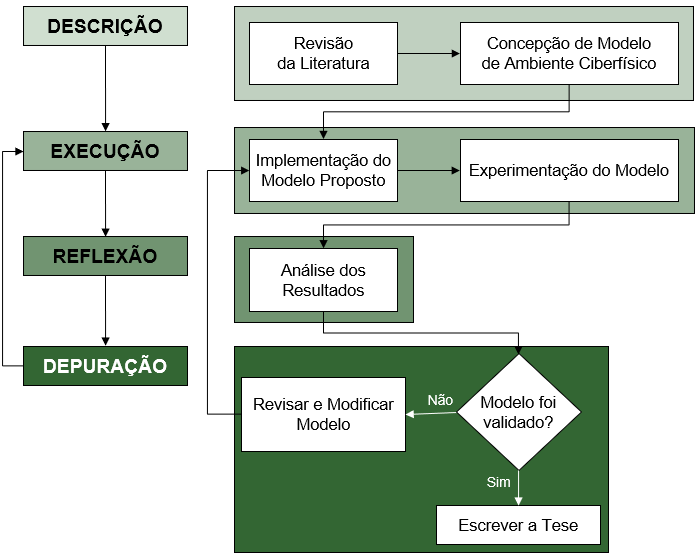
\includegraphics[width=0.8\linewidth]{imgs/METODOLOGIA_v2.png}
	\caption{Metodologia da pesquisa baseada no construcionismo de Papert}
	\label{fig:metodologia}
\end{figure}

%Com relação aos mapeamentos sistemáticos, foram planejados dois mapeamentos relativos a: (1) Recomendação de Recursos Pedagógicos utilizando sistemas computacionais cognitivos; (2) Implementação de ambientes de aprendizagem utilizando sistemas ciber-físicos. Tais mapeamentos seguem o método proposto por~\cite{kitchenham:2004} que consiste em três etapas~\citep{mafra:2006}: Planejamento do Mapeamento, Condução do Mapeamento, Análise e Publicação dos Resultados.

Ainda nessa fase, foi descrita a concepção da arquitetura e modelos do sistema proposto, tendo como base o ambiente de educação digital proposto no mestrado do proponente~\citep{leitao:2017}. Tal arquitetura foi expandida de modo a adicionar novas funcionalidades nos módulos existentes, tal como apresentado no Capítulo~\ref{Chap:prosedMethod}.

A fase de \textbf{Execução} é a fase de implementação e execução das ações descritas no Modelo com vistas a resolver o problema, além de realizar experimentos e observações para obtenção de resultados mensuráveis. Na fase de \textbf{Reflexão}, os resultados obtidos e os conceitos empregados são analisados e avaliados. Haverá também reflexão sobre os acertos, erros ou falhas ao longo do processo. A fase de \textbf{Depuração} visa revisar e, caso necessário, modificar a descrição e a implementação do Modelo fazendo ajustes para que o mesmo alcance os objetivos propostos. Assim, caso necessário, são novamente realizados as fases de ``Execução'' e ``Reflexão''.

\section{Abordagem Proposta}

Tendo em vista os desafios emanados da urgente necessidade de adaptação dos processos educacionais à nova realidade da Educação 4.0 de modo a incluir elementos de inteligência artificial, ciência de dados, internet das coisas e sistemas ciberfísicos no contexto educacional, com vistas a aprimorar as experiências de ensino-aprendizagem, tais como: a criação de ambientes de aprendizagem que incorporem elementos que tenham componentes que sejam físicos e digitais  e atuem de forma integrada; a coleta de dados de interação dos estudantes em ambos os componentes (físico e digital) de um objeto tangível; avaliação da aprendizagem através das experiências pedagógicas proporcionadas por objetos tangíveis de aprendizagem; e, a recomendação de objetos tangíveis de aprendizagem bem como a criação de padrões de metadados e de um repositório que permitam o reuso destes objetos.

%antigo Esta tese apresenta uma abordagem que expande o trabalho de mestrado de \cite{leitao:2017}, onde são propostas uma arquitetura e um conjunto de ferramentas que permitam a criação de uma aula com utilização de objetos físico-virtuais de aprendizagem, inclusive no processo de avaliação da aprendizagem. Assim, o método proposto nesta tese consiste de 5 componentes, sendo: (i) compositor: ferramenta para autoria de objetos físico-virtuais de aprendizagem que implementa uma proposta de modelo para estes objetos; (ii) servidor: \textit{middleware} para trocas de mensagens entre os componentes físicos e virtuais, além de recepção e consolidação dos dados coletados de interação dos estudantes com o material didático; (iii) player físico-virtual: interface de usuário para manipulação física ou virtual dos objetos de aprendizagem, sendo também responsável pela coleta dos dados de interação e seu envio ao servidor; (iv) analytics: módulo que implementa as métricas de avaliação da aprendizagem propostas nesta tese com o objetivo de gerar análises sobre as demandas dos estudantes; e, (v) inteligência: módulo baseado em agentes que recomendam objetos de aprendizagem ou notificam acerca das prioridades de tópicos ou disciplinas a ser estudados pelos alunos.

Esta tese apresenta uma abordagem
% que expande o trabalho de mestrado de \cite{leitao:2017},
onde são propostas uma arquitetura e um conjunto de ferramentas que permitam a criação de uma aula com utilização de objetos tangíveis de aprendizagem, inclusive no processo de avaliação da aprendizagem. Assim, o método proposto nesta tese consiste de quatro componentes, sendo: (i) compositor: ferramenta para autoria de objetos tangíveis de aprendizagem que implementa uma proposta de modelo para estes objetos; (ii) servidor: \textit{middleware} para trocas de mensagens entre os componentes físicos e digitais, além de recepção e consolidação dos dados coletados de interação dos estudantes com o material didático; (iii) player físico-virtual: interface de usuário para manipulação física ou digital dos objetos de aprendizagem, sendo também responsável pela coleta dos dados de interação e seu envio ao servidor; e, (iv) analíticos: módulo que implementa as métricas de avaliação da aprendizagem propostas nesta tese com o objetivo de gerar análises sobre as demandas dos estudantes.

Além disso, será apresentado um estudo de caso que servirá para validar e aprimorar a abordagem apresentada. Tal estudo de caso consiste na criação e utilização de um objeto tangível de aprendizagem baseado no método proposto que implementa o manipulativo ``quadro trigonométrico'' e proverá dados para análise da aprendizagem.

% -----------------------------------------------------------------
% => Organização do Trabalho
% -----------------------------------------------------------------
\section{Organização do Trabalho}
\label{section:outline}

A introdução deste trabalho apresentou o contexto, definição do problema, motivação e os objetivos desta pesquisa. Os capítulos restantes deste trabalho estão organizados da seguinte forma. 
No Capítulo~\ref{Chap:background}, \textbf{Conceitos e Definições}, são apresentados pressupostos pedagógicos e conceitos-chave abordados por este trabalho, tais como:
educação e práticas pedagógicas, as teorias sociopedagógicas, além de detalhes sobre a computação aplicada à educação.
%Educação e abordagens pedagógicas, o papel do professor no processo de ensino-aprendizagem, Computação Aplicada à Educação, Objetos de Aprendizagem, além de sistemas multiagente e sistemas ciber-físicos.
No Capítulo \ref{Chap:relatedWork}, \textbf{Trabalhos Correlatos}, são apresentados e discutidos alguns dos principais trabalhos relacionados ao uso de sistemas ciber-físicos em educação, além de ferramentas de autoria de objetos de aprendizagem e de avaliação da aprendizagem.
No Capítulo \ref{Chap:prosedMethod}, \textbf{Método Proposto}, são descritas a arquitetura e a abordagem propostas nesta Tese para criação de um ambiente de educação digital que suporte uma aula contendo objetos físico-virtuais de aprendizagem, além de permitir a avaliação da aprendizagem dos estudantes. Além disso, são também apresentadas as ferramentas desenvolvidas para implementação do estudo de caso que embasará a validação do método proposto.
%antigo No Capítulo~\ref{Chap:partialResults}, \textbf{Resultados Parciais}, são apresentados e analisados os resultados experimentais relacionados ao Módulo Analytics, onde as métricas de aprendizagem propostas nesta Tese são utilizadas para prover análises sobre os estudantes cujos dados de interação foram coletados. Além disso, são apresentadas uma proposta de estudo de caso relacionado a arquitetura proposta neste trabalho e dados acerca dos mapeamentos sistemáticos da literatura previstos na metodologia.
No Capítulo~\ref{Chap:Results}, \textbf{Resultados Experimentais}, são detalhadas as fases e os resultados do estudo de caso utilizado para validação da proposta apresentada neste trabalho.
% e dados acerca dos mapeamentos sistemáticos da literatura previstos na metodologia.
%No Capítulo \ref{Chap:partialResults}, \textbf{Resultados Experimentais}, são apresentados e analisados os resultados experimentais do método proposto. Na análise, são utilizadas métricas de aprendizagem que possibilitem verificar o desempenho \textit{a posteriori} dos estudantes no momento da execução da aula.
E, por fim, no Capítulo \ref{Chap:endFuture}, \textbf{Conclusões}, são expostas as considerações finais e os trabalhos futuros.